\documentclass{article}

\usepackage[utf8]{inputenc}
\usepackage{amsthm}
\usepackage{amssymb}
\usepackage{mathtools}
\usepackage{graphicx}
\usepackage{mdframed}
\usepackage{float}
\usepackage[top=0.75in, bottom=0.75in, left=0.75in, right=0.75in]{geometry}
\usepackage{gauss}

\usepackage{array}
\allowdisplaybreaks

\makeatletter
\newcounter{elimination@steps}
\newcolumntype{R}[1]{>{\raggedleft\arraybackslash$}p{#1}<{$}}
\def\elimination@num@rights{}
\def\elimination@num@variables{}
\def\elimination@col@width{}
\newenvironment{elimination}[4][0]
{
    \setcounter{elimination@steps}{0}
    \def\elimination@num@rights{#1}
    \def\elimination@num@variables{#2}
    \def\elimination@col@width{#3}
    \renewcommand{\arraystretch}{#4}
    \start@align\@ne\st@rredtrue\m@ne
}
{
    \endalign
    \ignorespacesafterend
}
\newcommand{\step}[2]
{
    \ifnum\value{elimination@steps}>0\sim\quad\fi
    \left[
        \ifnum\elimination@num@rights>0
            \begin{array}
            {@{}*{\elimination@num@variables}{R{\elimination@col@width}}
            |@{}*{\elimination@num@rights}{R{\elimination@col@width}}}
        \else
            \begin{array}
            {@{}*{\elimination@num@variables}{R{\elimination@col@width}}}
        \fi
            #1
        \end{array}
    \right]
    & 
    \begin{array}{l}
        #2
    \end{array}
    \addtocounter{elimination@steps}{1}
}
\makeatother

\DeclarePairedDelimiter{\abs}{\lvert}{\rvert}
\DeclarePairedDelimiter{\norm}{\lvert \lvert}{\rvert \rvert}

\newtheoremstyle{break}% name
  {}%         Space above, empty = `usual value'
  {}%         Space below
  {\itshape}% Body font
  {}%         Indent amount (empty = no indent, \parindent = para indent)
  {\bfseries}% Thm head font
  {.}%        Punctuation after thm head
  {\newline}% Space after thm head: \newline = linebreak
  {}%         Thm head spec

\newtheorem{Def}{Definition}[section]

\theoremstyle{break}

\newtheorem{innerEx}{Exempel}[section]
\newtheorem{sats}{Sats}[section]
\newtheorem{Rem}{Anmärkning}[]

\newenvironment{Ex}
{\begin{mdframed} \begin{innerEx} \vspace{3pt}}
{\vspace{3pt} \end{innerEx} \end{mdframed}}  

\newenvironment{bevis}
{\begin{mdframed} \begin{proof} \vspace{3pt}}
{\vspace{3pt} \end{proof} \end{mdframed}}


\title{
	 Linjär Algebra\\
	 Föreläsning 15 - Baser och basbyten
    \author{Erik Sjöström}
}
\begin{document}
\maketitle

\section{Basbyte} % (fold)
\label{sec:basbyte}
\begin{Ex}
	Låt $\vec{x} = \begin{bmatrix} 1\\6 \end{bmatrix}$, om vi använder standardbasen ($\vec{e}_1, \vec{e}_2 \in \mathbb{R}^^2$). Så menar vi:
	\[
	x = \begin{bmatrix} 1\\6 \end{bmatrix} = 1 \cdot \begin{bmatrix} 1\\0 \end{bmatrix} + 6 \cdot \begin{bmatrix} 0\\1 \end{bmatrix}
	\]
	\begin{center}
		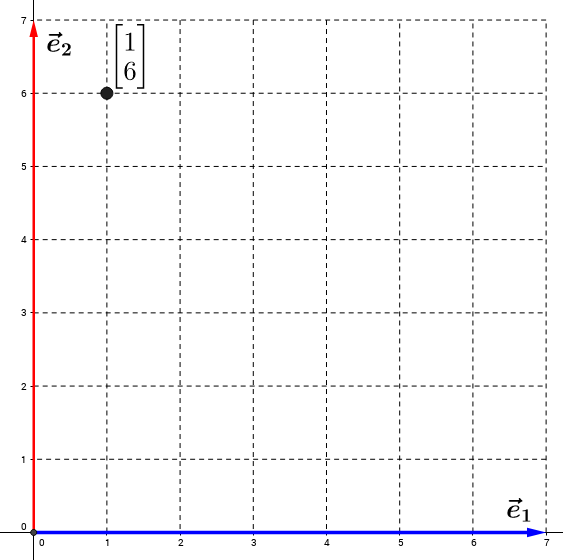
\includegraphics[scale=0.25]{ON.png}
	\end{center}
\end{Ex}
När vi anger en vektor så är det relativt en bas. Byter vi bas så ändras koordinaterna.
\begin{Ex}
	Låt:
	\begin{align*}
	&\vec{f}_1 = \begin{bmatrix} 1\\0 \end{bmatrix}
	&&\vec{f}_2 = \begin{bmatrix} 1\\2 \end{bmatrix}
	\end{align*}
	vara en bas i $\mathbb{R}^2$
	Låt $x_\mathbf{F} = \begin{pmatrix} -2\\3 \end{pmatrix}$ vara en punkt uttryckt i \textbf{F}-basen.
	\begin{center}
		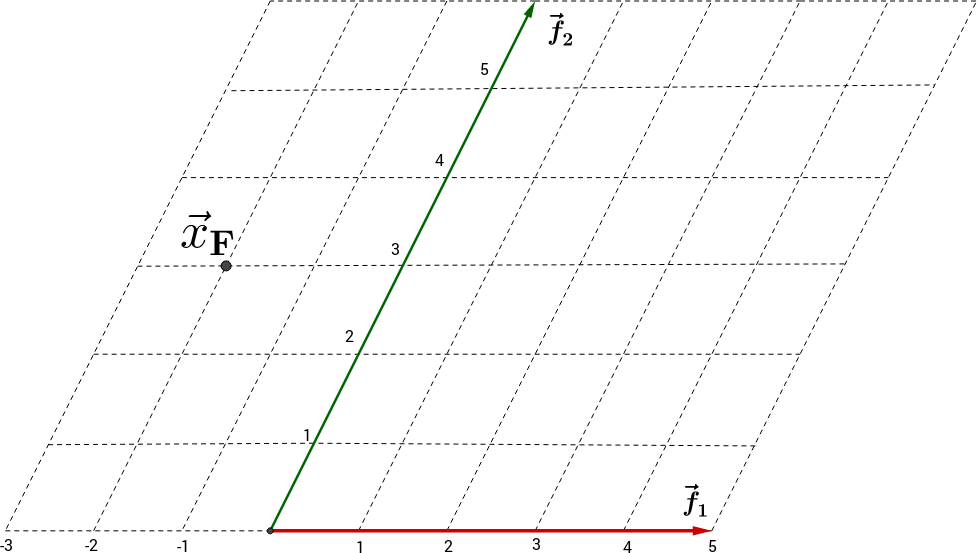
\includegraphics[scale=0.25]{egen.png}
	\end{center}
	Bestäm $\vec{x}_\mathbf{F}$ i basen ($\vec{e}_1, \vec{e}_2$):
	\begin{gather*}
		\vec{x}_\mathbf{F]} = 
		\overbrace{\begin{bmatrix} 1\\0 \end{bmatrix}}^{\vec{f}_1} \cdot -2 + 
		\overbrace{\begin{bmatrix} 1\\2 \end{bmatrix}}^{\vec{f}_2} 
		\cdot 3 = x_1 \vec{e}_1 + x_2 \vec{e}_2 = \vec{x}\\
		\begin{bmatrix} 1&1\\0&2 \end{bmatrix} \begin{bmatrix} -2\\3 \end{bmatrix} = \begin{bmatrix} x_1\\x_2 \end{bmatrix} 
		\Leftrightarrow 
		\begin{cases}
			x_1 = 1\\
			x_2 = 6
		\end{cases}
	\end{gather*}
	dvs $\vec{x}_\mathbf{F}$ uttryckt i ($\vec{e}_1, \vec{e}_2$) är: $\begin{bmatrix} 1\\6 \end{bmatrix}$\\
	\paragraph{-} % (fold)
	\label{par:_}
	Bestäm $(\vec{e}_2)_\mathbf{F}$ (bestäm $\begin{bmatrix} 0\\1 \end{bmatrix}$ i basen $\mathbf{F}$)
	\begin{gather*}
		\vec{e}_2 = 0 \cdot \overbrace{\begin{bmatrix} 1\\0 \end{bmatrix}}^{\vec{e}_1} + 1 \cdot \overbrace{\begin{bmatrix} 0\\1 \end{bmatrix}}^{\vec{e}_2} = x_1 \cdot \overbrace{\begin{bmatrix} 1\\0 \end{bmatrix}}^{\vec{f}_1} + x_2 \cdot \overbrace{\begin{bmatrix} 1\\2 \end{bmatrix}}^{\vec{f}_2} \Leftrightarrow\\
		\begin{bmatrix} 0\\1 \end{bmatrix} = \begin{bmatrix} 1&1\\0&2 \end{bmatrix} \begin{bmatrix} x_1\\x_2 \end{bmatrix} \Leftrightarrow \begin{bmatrix}
		\begin{array}{cc|c}
		    1&1&0\\
		    0&2&1
		\end{array}
		\end{bmatrix} \Rightarrow
		\begin{cases}
			x_1 = -1/2\\
			x_2 = 1/2
		\end{cases}
	\end{gather*}
	Vi har alltså $(\vec{e}_2)_\mathbf{F} = \begin{bmatrix} -1/2\\1/2 \end{bmatrix}$
	% paragraph _ (end)
\end{Ex}
Basbyten mellan $(\vec{e}_1, \vec{e}_2,...,\vec{e}_n)$ och ($\vec{f}_1, \vec{f}_2,...,\vec{f}_n$) i $\mathbb{R}^n$ ges a v följande:
\[
\overbrace{\begin{bmatrix} \vec{f}_1 & \vec{f}_2 &...&\vec{f}_n \end{bmatrix}}^\text{\textbf{F}: basbytesmatris} \cdot \vec{u}_{\mathbf{F}} = \vec{u}
\]
där $\vec{u}_F$ är koordinaterna av $\vec{u}$ i basen \textbf{F}.
\section{Räkneregler} % (fold)
\label{sec:r_kneregler}
\begin{align*}
&\mathbf{F} \cdot \vec{u}_{\mathbf{F}} = \vec{u}
&&\mbox{och}
&&\mathbf{F}^{-1} \cdot \vec{u} = \vec{u}_\mathbf{F}
\end{align*}
\textbf{F} är inverterbar ty kolumnerna i \textbf{F} är \textit{n} stycken linjärt oberoende vektorer i $\mathbb{R}^n$
\paragraph{-} % (fold)
\label{par:_2}
Låt $\mathbf{F} = \begin{bmatrix} \vec{f}_1 & \vec{f}_2 & ... & \vec{f}_n \end{bmatrix}$ och $\mathbf{G} = \begin{bmatrix} \vec{g}_1 & \vec{g}_2 & ... & \vec{g}_n \end{bmatrix}$.\\
Låt $\vec{x}$ vara en vektor med koordinaten $\vec{x}_\mathbf{F}$ i basen \textbf{F} och $\vec{x}_\mathbf{G}$ i basen \textbf{G}, då gäller:
\[
\text{Basbytesformeln}: 
\begin{cases}
	\mathbf{G} \cdot \vec{x}_{\mathbf{G}} = \mathbf{F} \cdot \vec{x}_\mathbf{F}\\
	\vec{x}_{\mathbf{G}} = \mathbf{G}^{-1} \cdot \mathbf{F} \cdot \vec{x}_{\mathbf{F}}\\
	\vec{x}_{\mathbf{F}} = \mathbf{F}^{-1} \cdot \mathbf{G} \cdot \vec{x}_{\mathbf{G}}
\end{cases}
\]
\begin{Ex}
	Låt:
	\begin{align*}
	&\mathbf{F} = \begin{bmatrix} 1&-1\\1&1 \end{bmatrix}
	&&\text{och}
	&&\mathbf{G} = \begin{bmatrix} -1&-1\\1&-1 \end{bmatrix}
	\end{align*}
	vara två matriser vars kolumner bildar två olika baser i $\mathbb{R}^2$
	\begin{center}
		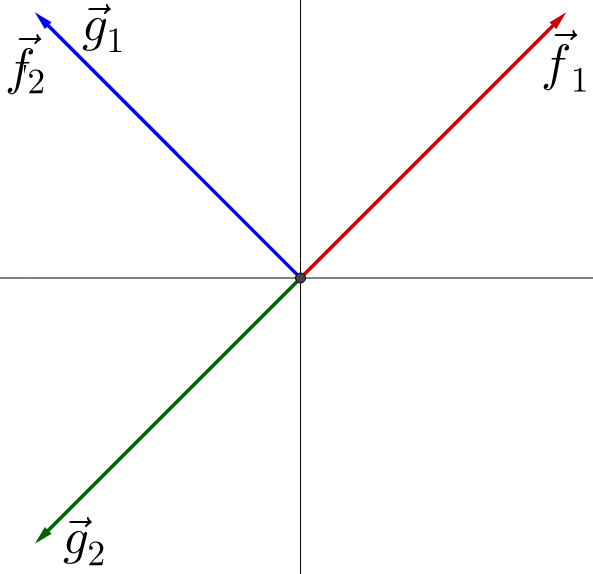
\includegraphics[scale=0.25]{baser.png}
	\end{center}
	Antag $\vec{v}_{\mathbf{F}} = \begin{bmatrix} 2\\3 \end{bmatrix}$, bestäm $\vec{v}_{\mathbf{G}}$
	\begin{gather*}
		\mathbf{F} \cdot \vec{v}_{\mathbf{F}} = \begin{bmatrix} 1 & -1\\1 & 1 \end{bmatrix} \begin{bmatrix} 2\\3 \end{bmatrix} = \begin{bmatrix} -1\\5 \end{bmatrix}\\
		\vec{v}_{\mathbf{G}} = \mathbf{G}^{-1} \cdot \begin{bmatrix} -1\\5 \end{bmatrix} \Leftrightarrow \mathbf{G} \cdot \vec{v}_{\mathbf{G}} = \begin{bmatrix} -1\\5 \end{bmatrix}
	\end{gather*}
	Dvs:
	\[
	\begin{bmatrix}
	\begin{array}{cc|c}
	    -1 & -1 & -1\\
	    1 & -1 & 5
	\end{array}
	\end{bmatrix}
	\sim .. \sim
	\begin{bmatrix}
	\begin{array}{cc|c}
	    1 & 1 & 1\\
	    0 & 1 & -2
	\end{array}
	\end{bmatrix}
	\Rightarrow
	\begin{cases}
		x_1 = 3\\
		x_2 = -2
	\end{cases}
	\]
	Dvs:
	\[
	\vec{v}_{\mathbf{G}} = \begin{bmatrix} 3\\-2 \end{bmatrix}
	\]
\end{Ex}
\section{Baser} % (fold)
\label{sec:baser}
En bas $(\vec{v}_1, \vec{v}_2,...,\vec{v}_n$ är en ON-bas för $\mathbb{R}^n$ om vektorerna $\vec{v}_1, \vec{v}_2,...,\vec{v}_n$ är parvis ortogonala och har längden 1. Dvs:
\[
\vec{v}_i \cdot \vec{v}_j = 
\begin{cases}
	1 \text{ om } i = j\\
	0 \text{ om } i \neq j
\end{cases}
\]
(om ett antal vektorer är parvis ortogonala så är de linjärt oberoende)
\begin{Ex}
	\begin{align*}
	&\vec{e}_1 = \begin{bmatrix} 1\\0\\0 \end{bmatrix}
	&&\vec{e}_2 = \begin{bmatrix} 0\\1\\0 \end{bmatrix}
	&&\vec{e}_3 = \begin{bmatrix} 0\\0\\1 \end{bmatrix}
	\end{align*}
	är en ON-bas för $\mathbb{R}^3$. Vi ser att:
	\begin{align*}
	&\vec{e}_1 \cdot \vec{e}_1 = 1
	&&\vec{e}_1 \cdot \vec{e}_2 = 0
	&&\vec{e}_1 \cdot \vec{e}_3 = 0
	\\
	&\vec{e}_2 \cdot \vec{e}_2 = 1
	&&\vec{e}_2 \cdot \vec{e}_3 = 0
	\\
	&\vec{e}_3 \cdot \vec{e}_3 = 1
	\end{align*}
\end{Ex}

\begin{Ex}
	$\begin{bmatrix} 1\\0 \end{bmatrix}$, $\begin{bmatrix} 1\\2 \end{bmatrix}$ är en bas i $\mathbb{R}^2$ (ty de är ej linjärt oberoende). Men ej en ON-bas, ty:
	\[
	\begin{bmatrix} 1\\0 \end{bmatrix} \cdot \begin{bmatrix} 1\\2 \end{bmatrix} = 1 \neq 0
	\]
\end{Ex}
\section{Isometriska avbildningar} % (fold)
\label{sec:isometriska_avbildningar}
\begin{Def}
	En linjär avbildning $f:\mathbb{R}^n \rightarrow \mathbb{R}^n$, $f(\vec{x}) = \mathbf{A} \cdot \vec{x}$ är \underline{isometrisk} om den bevarar längden. Dvs:
	\[
	\norm{f(\vec{x})} = \norm{\mathbf{A} \cdot \vec{x}} = \norm{\vec{x}} \text{\hspace{7pt}} \forall \vec{x} \in \mathbb{R}^n
	\]
\end{Def}

\begin{Ex}
	Rotation bevara längden.
\end{Ex}

Vad innebär det för \textbf{A} (avbildningsmatrisen) att \textit{f} är isometriskt?. Låt:
\[
\vec{x} = \begin{bmatrix} x_1\\x_2\\\vdots\\x_n \end{bmatrix}
\]
Vi har att:
\begin{gather*}
	\norm{\vec{x}}^2 = \vec{x}_1^2 + \vec{x}_2^2 + ... + \vec{x}_n^2 = \begin{bmatrix} x_1 & x_2 & ... & x_n \end{bmatrix} \begin{bmatrix} x_1\\x_2\\\vdots\\x_n \end{bmatrix} = \vec{x}^T \cdot \vec{x}\\
	\overbrace{\norm{f(\vec{x})}^2}^\text{Längden av bilden} = \norm{\mathbf{A} \cdot \vec{x}}^2 = (\mathbf{A} \cdot \vec{x})^T \cdot (\mathbf{A} \cdot \vec{x}) = \text{ Matrisvektorproduktregler }
	= (\vec{x}^T \cdot \mathbf{A}^T) \cdot (\mathbf{A} \cdot \vec{x}) = \vec{x}^T \cdot \overbrace{\mathbf{A}^T \cdot \mathbf{A}}^\mathbf{B} \cdot \vec{x}
\end{gather*}
Eftersom $\mathbf{A}^T \cdot \mathbf{A}$ är symmetrisk och den ända symmetriska matris som uppfyller villkoret är $\mathbf{B} = \mathbf{I}$ (identitetsmatrisen) så måste $\mathbf{A}^T \cdot \mathbf{A} = \mathbf{I}$. Dvs kolumnerna i \textbf{A} är parvis ortogonala.
\[
\vec{a}_i \cdot \vec{a}_j = 
\begin{cases}
	1 \text{ om } i = j\\
	0 \text{ om } i \neq j
\end{cases}
\]
En linjär avbildning är isometrisk då avbildningsmatrisens kolumn utgör en ON-bas. En sådan matris kallas för ON-matris.
\begin{Ex}
	Rotation är en isometrisk avbildning $f:\mathbb{R}^2 \rightarrow \mathbb{R}^2$
	\[
	f(\vec{x}) =
	\overbrace{
	\begin{bmatrix}
		\cos(\theta) & -\sin(\theta)\\
		\sin(\theta) & \cos(\theta)
	\end{bmatrix}
	}^\mathbf{A}
	\begin{bmatrix} x_1\\x_2 \end{bmatrix}
	\]
	Eftersom:
	\begin{align*}
	\mathbf{A}^T \cdot \mathbf{A} &=
	\begin{bmatrix}
		\cos(\theta) & \sin(\theta)\\
		-\sin(\theta) & \cos(\theta)
	\end{bmatrix}
	\begin{bmatrix}
		\cos(\theta) & -\sin(\theta)\\
		\sin(\theta) & \cos(\theta)
	\end{bmatrix}
	\\
	&=
	\begin{bmatrix}
		\cos^2(\theta) + \sin^2(\theta) & -\cos(\theta) \cdot \sin(\theta) + \sin(\theta) \cdot \cos(\theta)\\
		-\sin(\theta) \cdot \cos(\theta) + \cos(\theta) \cdot \sin(\theta) & \cos^2(\theta) + \sin^2(\theta)
	\end{bmatrix}
	\\
	&=
	\begin{bmatrix} 1&0\\0&1 \end{bmatrix}
	\end{align*}
\end{Ex}
Om \textbf{A} är ON-matris så gäller också att:
\[
(\mathbf{A} \cdot \vec{x}) \cdot (\mathbf{A} \cdot \vec{y}) = \vec{x} \cdot \vec{y}
\]
för $\vec{x}$, $\vec{y}$ $\in \mathbb{R}^n$. Dvs den isometriska avbildningen bevarar även vinklar. Vinkeln mellan $f(\vec{x})$ och $f(\vec{y})$ är samma som mellan $\vec{x}$ och $\vec{y}$
\paragraph{Vinkeln i $\mathbb{R}^n$} % (fold)
  \label{par:vinkeln_i_}
  (rep)
  \[
  \cos(\theta) = \frac{\vec{x} \cdot \vec{y}}{\norm{\vec{x}} \cdot \norm{\vec{y}}}
  \]
  % paragraph vinkeln_i_ (end)
\begin{sats}
	Om \textbf{A} är en ON-matris så är $\mathbf{A}^T = \mathbf{A}^{-1}$:
\end{sats}\\
\begin{bevis}
	Vill visa att:
\[
\begin{cases}
  	\mathbf{A} \cdot \mathbf{B} = \mathbf{I}\\
  	\mathbf{B} \cdot \mathbf{A} = \mathbf{I}
  \end{cases}  
\]  
Vi vet att:
\[
\begin{cases}
	\mathbf{A} \cdot \mathbf{A}^T = \mathbf{I}\\
	\mathbf{A}^T \cdot \mathbf{A} = \mathbf{I}
\end{cases}
\]
Så:
\[
\mathbf{A} \cdot \mathbf{A}^T = \mathbf{C} \Rightarrow \mathbf{A} \cdot \overbrace{\mathbf{A}^T \cdot \mathbf{A}}^\mathbf{I} = \overbrace{\mathbf{C}}^\mathbf{I} \cdot \mathbf{A}
\]
\end{bevis}
% section isometriska_avbildningar (end)

% section baser (end)

\end{document}